\chapter{Ergebnisse}
\label{chap:berechnung}
Der Hamiltonian des betrachteten Graphens mit Mn-Defekt bei Vernachlässigung der Coulomb-Wechselwirkung zwischen den Elektronen lautet
\begin{align*}
   H &=  H_0 + H_\text{Def} + H_\text{Kop}\\
    &=- t \sum_{i=1}^N \sum_{j=1}^N\left ( c_i^\dagger c_j + c_j^\dagger c_i \right )  + \sum_{m=1}^5 \epsilon_m d_m^\dagger d_m
    + \sum_{m=1}^5 \sum_{j=1}^3 \left ( V_{mj} d_m^\dagger c_j + \overline{V}_{mj} c_j^\dagger d_m \right )  \; \text{.} \numberthis \label{eqn:full_Hamiltonian}
\end{align*}
Die Summation über $N$ Basen in dem Term $H_0$ läuft nur über nächste Nachbarn.
Der Vernichter(Erzeuger) $c_i(c_i^{\dagger})$ vernichtet(erzeugt) ein Elektron im $p_z$-Orbital am Gitterplatz $i$.
Damit wird mit dem Hüpfparameter $t$ das Hüpfen zwischen nächsten Nachbarn des ungestörten Graphengitters beschrieben.
Aufgrund der Periodizität und der ausschließlichen Betrachtung des Hüpfens zwischen $p_z$-Orbitale, ist der  
Hüpfparameter $t$ für alle Summanden gleich.   
Die Störstelle wird mit dem Hamiltonian $H_\text{Def}$ umfasst. 
Der Vernichter(Erzeuger) $d_m(d_m^{\dagger})$ vernichtet(erzeugt) dabei ein Elektron in dem $m$-ten $3d$-Orbital mit der 
Orbitalenergie $\epsilon_m$ \cite{anders-fkt}.
In dem letzten Term des Hamiltonians, $H_\text{Kop}$, wird die Kopplung der $3d$-Orbitale des Mn und 
den $p_z$-Orbitalen der drei umliegenden C (siehe Abbildung \ref{fig:mangan_impurity_inplane}) aufgefasst.
Die auftretenden Hüpfparameter sind nicht wie zuvor bei $H_0$ für alle Summanden gleich, da fünf verschiedene Orbitale
des Mn und die verschiedenen räumlichen Anordnungen der drei umliegenden C einen Einfluss haben.
Somit bezeichnet $V_{mj}$ das SK-Integral für das Hüpfen zwischen dem $m$-ten $3d$-Orbital des Mn mit dem $p_z$-Orbital des 
$j$-ten benachbarten C.
Da die SK-Integrale reell sind, folgt $\overline{V}_{mj} = V_{mj}$.
Sofern es eindeutig ist, wird im Folgenden auf explizite Angabe des Startwerts des Laufindex und der oberen Grenze bei Summationen verzichtet.
\section{Slater-Koster-Integrale}
\label{sec:slaterkostercalc}
Zur Berechnung der SK-Integrale werden die Richtungskosinus \eqref{eqn:RK} benötigt.
Der Betrag des Abstandsvektors (siehe Abschnitt \ref{sec:structure}) für das $j$-te der drei umligenden C um das Mn ist durch 
\begin{equation}
    \left | \vec{d}_j  \right | = a \sqrt{\cos^2(\varphi_j) + \sin^2(\varphi_j) + \cot^2(\theta)} = a \sqrt{1+\cot^2(\theta)} = \frac{a}{\sin(\theta)} \label{eqn:distance}
\end{equation}
gegeben.
In Gleichung \eqref{eqn:distance} wurde zur Vereinfachung des Abstands die trigonometrische Beziehung $ \sin(\theta)^{-1} = \sqrt{1+\cot^2(\theta)}$ \cite{trig} mit der Beschränkung
$\theta \in ( 0, \sfrac{\pi}{2} ] $ ausgenutzt. 
Diese Beschränkung ist jedoch gerechtfertigt, da das Mn nur unterhalb des Graphens und mittig von den drei umliegenden C betrachtet wird.
Die Skalarprodukte ausgewertet und der Abstand eingesetzt ergibt
\begin{equation*}
    l = \cos(\varphi_j) \sin(\theta) \; , \quad
    m = \sin(\varphi_j) \sin(\theta) \; , \quad
    n = \cot(\theta) \sin(\theta) = \cos(\theta) \; .
\end{equation*}
Diese Ausdrücke für die Richtungskosinus werden in die SK-Integrale für die Kopplung zwischen den drei umliegenden 
$p_z$-Orbitale der C und den fünf $3d$-Orbitalen des Mn (siehe Anhang \ref{TEMPLATE}) eingesetzt,
so dass sich die Werte in Tabelle \ref{tab:slaterkosters} ergeben.
\begin{table}
    \centering
    \caption{SK-Integrale für den Überlapp der $p_z$-Orbitale des $j$-ten umliegenden
    C und der fünf $3d$-Orbitale des Mn in Abhängigkeit des Winkels $\theta$.}
    \label{tab:slaterkosters}
    \begin{tabular}{l c c c}
    & \multicolumn{3}{c}{$j$-tes C}\\
    \cmidrule(lr){2-4}
    & {$1$} & {$2$} & {$3$} \\
    \midrule
    {$E_{z,xy}$      }  & {$0$}                                               & {$-\frac{3}{4}bV_{pd\sigma} + \frac{\sqrt{3}}{2}bV_{pd\pi}$}          & {$ \frac{3}{4}bV_{pd\sigma}-\frac{\sqrt{3}}{2}bV_{pd\pi}$}         \vspace{0.5cm} \\ 
    {$E_{z,xz}$      }  & {$\sqrt{3}fV_{pd\sigma} + hV_{pd\pi}$}              & {$-\frac{\sqrt{3}}{2}fV_{pd\sigma} - \frac{1}{2} hV_{pd\pi}$}         & {$-\frac{\sqrt{3}}{2}fV_{pd\sigma} - \frac{1}{2} hV_{pd\pi}$}      \vspace{0.5cm} \\
    {$E_{z,zy}$      }  & {$0$}                                               & {$ \frac{3}{2}fV_{pd\sigma}+\frac{\sqrt{3}}{2} hV_{pd\pi}$}           & {$-\frac{3}{2}fV_{pd\sigma}-\frac{\sqrt{3}}{2} hV_{pd\pi}$}        \vspace{0.5cm} \\
    {$E_{z,3z^2-r^2}$}  & {$q V_{pd\sigma}+\sqrt{3}bV_{pd\pi}$}               & {$q V_{pd\sigma}+\sqrt{3}bV_{pd\pi}$}                                 & {$q V_{pd\sigma}+\sqrt{3}bV_{pd\pi}$} \vspace{0.5cm} \\
    {$E_{z,x^2-y^2}$ }  & {$\frac{\sqrt{3}}{2}bV_{pd\sigma}-bV_{pd\pi}$}      & {$-\frac{\sqrt{3}}{4}bV_{pd\sigma}+\frac{1}{2}bV_{pd\pi}$}           & {$-\frac{\sqrt{3}}{4}bV_{pd\sigma}+\frac{1}{2}bV_{pd\pi}$}                       \\ 
    \bottomrule
    \end{tabular}
  \end{table}
Um die Übersichtlichkeit zu gewährleisten, wurden die von dem Winkel $\theta$ abhängigen Koeffizienten zu
\begin{equation}
    \begin{aligned}
b & \coloneq -\sin^2(\theta) \cos(\theta)        & f &  \coloneq -\cos^2(\theta) \sin(\theta)                             \\                     
h & \coloneq -\sin(\theta)(1-2\cos^2(\theta))    & q &  \coloneq -\cos^3(\theta) + \frac{1}{2}\sin^2(\theta) \cos(\theta)
    \end{aligned} \label{eqn:Vorfaktoren}
\end{equation}
umdefiniert.
\section{Hybridisierungsfunktion}
\label{sec:calc_greensfunction}
Aufgrund der Gitterperiodizität kann für die Operatoren $c_i$ (Untergitter A) und $c_j$ (Untergitter B) eine Fouriertransformation der Form 
\begin{equation}
    c_i = \frac{1}{\sqrt{N}} \sum_{\vec{k}}^{1. \, \text{BZ}} \symup{e}^{\symup{i}\vec{k}\vec{l}} c_{\text{A}, \vec{k}} \; , 
    \quad c_j = \frac{1}{\sqrt{N}} \sum_{\vec{k}}^{1. \, \text{BZ}} \symup{e}^{\symup{i}\vec{k}(\vec{l}+\vec{\delta}_j)} c_{\text{B}, \vec{k}} \label{eqn:fourier_ladder}
\end{equation}
angesetzt werden.
Dabei sind $N$ die Anzahl der Basen, $\vec{l}$ der Gittervektor der Basis, $\vec{k}$ der Wellenvektor, $\vec{\delta}_j$ der Abstandsvektor
des $j$-ten C auf dem Untergitter B, welches eins der drei nächsten Nachbarn des C auf dem Untergitter A mit dem Gittervektor $\vec{l}$ ist 
und $c_{A, \vec{k}}$ bzw. $c_{B, \vec{k}}$ die Fourier-transformierten $p_z$-Orbitale auf dem Untergitter A bzw. B \cite{anders-fkt}.
Die $\vec{k}$-Werte werden aus der ersten Brillouin-Zone genommen \cite{anders-fkt}.
Damit lässt sich der Hamiltonian des ungestörten Graphens zu 
\begin{align*}
    H_0 &= -\frac{t}{N} \sum_{j\vec{l}} \sum_{\vec{k}\vec{k}'} ( \symup{e}^{-\symup{i}\vec{k}\vec{l}}c^\dagger_{A,\vec{k}} 
    \symup{e}^{\symup{i}\vec{k}'(\vec{l}+\vec{\delta}_j)}c_{B,\vec{k}'} + \symup{e}^{-\symup{i}\vec{k}'(\vec{l}+\vec{\delta}_j)} c^\dagger_{B,\vec{k}'} 
    \symup{e}^{i\vec{k}\vec{l}}c_{A,\vec{k}}) \\
    &= -\frac{t}{N} \sum_{j\vec{l}} \sum_{\vec{k}\vec{k}'} ( \symup{e}^{-\symup{i}(\vec{k}- \vec{k}')\vec{l}}\symup{e}^{\symup{i}\vec{k'}\vec{\delta}_j}c^\dagger_{A,\vec{k}} c_{B,\vec{k}'} + 
    \symup{e}^{\symup{i}(\vec{k}- \vec{k}')\vec{l}} \symup{e}^{-\symup{i}\vec{k'}\vec{\delta}_j} c^\dagger_{B,\vec{k}'}c_{A,\vec{k}}) \\
    &= -t \sum_{j\vec{k}} ( \symup{e}^{\symup{i}\vec{k}\vec{\delta}_j}c^\dagger_{A,\vec{k}} c_{B,\vec{k}} + 
    \symup{e}^{-\symup{i}\vec{k}\vec{\delta_j}} c^\dagger_{B,\vec{k}}c_{A,\vec{k}})
\end{align*}
schreiben.
In dem letzten Schritt wurde $\sum_{\vec{l}}^N \symup{e}^{-i(\vec{k}- \vec{k}')\vec{l}} 
= \sum_{\vec{l}}^N \symup{e}^{i(\vec{k}- \vec{k}')\vec{l}} = N\delta_{\vec{k}, \vec{k}'}$ ausgenutzt, so dass die Summe über $\vec{k}'$ verschwindet.
In $H_\text{Kop}$ werden die transformierten Erzeuger ohne weitere Vereinfachungen eingesetzt,  so dass der Gesamthamiltonian zu 
\begin{equation*}
    \begin{split}
        H = &-t \sum_{j \vec{k}} ( \symup{e}^{\symup{i}\vec{k}\vec{\delta}_j}c^\dagger_{A,\vec{k}} c_{B,\vec{k}} + 
            \symup{e}^{-\symup{i}\vec{k}\vec{\delta}_j} c^\dagger_{B,\vec{k}}c_{A,\vec{k}}) + \sum_m \epsilon_m d_m^\dagger d_m \\
            &+ \frac{1}{\sqrt{N}}\sum_{mj\vec{k}} ( V_{mj}  \symup{e}^{\symup{i}\vec{k}(\vec{l}+\vec{\delta}_j)} d_m^\dagger c_{\text{B},\vec{k}} 
            + V_{mj} \symup{e}^{-\symup{i}\vec{k}(\vec{l}+\vec{\delta}_j)}c^\dagger_{\text{B},\vec{k}} d_m )
    \end{split}
\end{equation*}
bestimmt werden kann.
Auf welchem Gitterplatz das Mn sitzt, wurde hierbei variabel gelassen.
Jedoch macht es in dieser Modellierung keinen Unterschied, welche Position das Mn einnimmt, wie sich im Verlauf der Berechnung auch zeigt.
Nun können die Einträge der gesuchten Matrix $\underline{\underline{G}}$ mit Hilfe der Bewegungsleichung \eqref{eqn:fouriereom} 
\begin{equation}
    zG_{d_m, d_{m'}^\dagger}(z) = \langle \{ d_m, d_{m'}^\dagger \} \rangle - G_{[H,d_m], d_{m'}^\dagger} (z) \label{eqn:eomgreenansatz}
\end{equation}
bestimmt werden.
Da sich das Argument der Greensche Funktion nicht ändert, wird im Folgenden drauf verzichtet, das Argument mit anzugeben.
Dazu wird der Kommutator $[H,d_m]$ aufgrund der Linearität in drei einzelne Kommutatoren unterteilt, so dass
\begin{equation*}
    [H,d_m] = [H_0,d_m] + [H_\text{Def},d_m] +[H_\text{Kop},d_m] 
\end{equation*}
berechnet werden muss.
Somit lautet der gesamte Kommutator
\begin{equation}
    \begin{split}
    [H, d_m] = &-t \sum_{j\vec{k}} \left ( \symup{e}^{\symup{i}\vec{k} \vec{\delta}_j}      \left [ c^\dagger_{\text{A},\vec{k}}  
        c_{\text{B},\vec{k}}, d_m \right ] + \symup{e}^{-\symup{i}\vec{k} \vec{\delta}_j}   \left [ c^\dagger_{\text{B},\vec{k}}  
        c_{\text{A},\vec{k}}, d_m \right ]  \right ) \\
        &+\sum_{m'} \varepsilon_{m'} \left [ d^\dagger_{m'} d_{m'}, d_{m} \right ] \\
        &+ \frac{1}{\sqrt{N}} \sum_{m'j\vec{k}} \left ( V_{m'j} \symup{e}^{\symup{i}\vec{k} (\vec{l} + \vec{\delta}_j)}   
        \left [d^\dagger_{m'}c_{\text{B}, \vec{k}}, d_m \right ]
        +  V_{m'j} \symup{e}^{-\symup{i}\vec{k} (\vec{l} + \vec{\delta}_j)}   
        \left [c^\dagger_{\text{B},\vec{k}} d_{m'},  d_m \right ]
        \right ) \; . \label{eqn:commutator_H_dm}
    \end{split}
\end{equation} 
Die Kommutatoren werden im Folgenden separat ausgerechnet, damit diese hinterher nur noch eingesetzt werden müssen.
Für den ersten Kommutator folgt
\begin{equation}
    \left [ c^\dagger_{\text{A},\vec{k}}  c_{\text{B},\vec{k}}, d_m \right ]  = c^\dagger_{\text{A},\vec{k}}  c_{\text{B},\vec{k}}  d_m 
        -  d_m c^\dagger_{\text{A},\vec{k}}  c_{\text{B},\vec{k}}
        = - c^\dagger_{\text{A},\vec{k}} d_m c_{\text{B},\vec{k}} + c^\dagger_{\text{A},\vec{k}} d_m c_{\text{B},\vec{k}} = 0 \label{eqn:kommutatornull} \; .
\end{equation}
Bei dem Kommutator $\left [ c^\dagger_{\text{B},\vec{k}} c_{\text{A},\vec{k}}, d_m \right ]$ ist die Vorgehensweise und das Ergebnis gleich,
so dass auf ein explizites Vorrechnen verzichtet wird.
Weiterhin wird 
\begin{align*}
    \left [ d^\dagger_{m'} d_{m'}, d_{m} \right ] &= d^\dagger_{m'} d_{m'} d_{m} - d_{m} d^\dagger_{m'} d_{m'}  =
    - d^\dagger_{m'} d_{m} d_{m'} - \delta_{mm'} d_{m'} +  d^\dagger_{m'} d_{m} d_{m'} \\
    &= - \delta_{mm'} d_{m'}
\end{align*} 
berechnet.
Die Kommutatoren mit den Operatoren in $H_\text{Kop}$ ergeben 
\begin{align*}
    \left [d^\dagger_{m'} c_{\text{B},\vec{k}}, d_m \right ] &= d^\dagger_{m'} c_{\text{B},\vec{k}} d_m -d_m d^\dagger_{m'}c_{\text{B}, \vec{k}} 
    = - d^\dagger_{m'} d_m c_{\text{B},\vec{k}} - \delta_{mm'} c_{\text{B},\vec{k}} + d^\dagger_{m'} d_m c_{\text{B},\vec{k}} \\
    &= - \delta_{mm'} c_{\text{B},\vec{k}}
\end{align*}
und 
\begin{equation}
    \left [c^\dagger_{\text{B},\vec{k}} d_{m'},  d_m \right ] = c^\dagger_{\text{B},\vec{k}} d_{m'} d_m - d_m c^\dagger_{\text{B},\vec{k}} d_{m'} 
    = - c^\dagger_{\text{B},\vec{k}} d_{m} d_{m'} + c^\dagger_{\text{B},\vec{k}} d_m  d_{m'} = 0 \; . \label{eqn:commutatornulldagger}
\end{equation}
Werden nun alle eben berechneten Kommutatoren in \eqref{eqn:commutator_H_dm} eingesetzt, folgt mittels Auswertung der Kronecker-Delta
\begin{align*}
        [H, d_m] =& -\sum_{m'} \varepsilon_{m'} \delta_{mm'} d_{m'} - 
        \frac{1}{\sqrt{N}} \sum_{m'j\vec{k}} V_{m'j} \symup{e}^{\symup{i}\vec{k} (\vec{l} + \vec{\delta}_j)}  \delta_{mm'} c_{\text{B}, \vec{k}} \\
        = &- \varepsilon_m d_m - \frac{1}{\sqrt{N}} \sum_{j\vec{k}} V_{mj} \symup{e}^{\symup{i}\vec{k} (\vec{l} + \vec{\delta}_j)} c_{\text{B}, \vec{k}} \; .
        \numberthis \label{eqn:commutator_H_dm_eingesetzt}
\end{align*}
Die Summationen über $m'$ sind in Gleichung \eqref{eqn:commutator_H_dm_eingesetzt} aufgrund der Kronecker-Delta entfallen.
Der somit berechnete Kommutator kann in die ursprüngliche Bewegungsleichung \eqref{eqn:eomgreenansatz} eingesetzt werden, woraus mit 
$\langle \{ d_m, d_{m'}^\dagger \} \rangle = \delta_{mm'}$ und Gleichung \eqref{eqn:commutator_H_dm_eingesetzt}
\begin{align*}
    z&G_{d_m, d_{m'}^\dagger} = \delta_{mm'} + \varepsilon_m G_{d_m, d^\dagger_{m'}} + \frac{1}{\sqrt{N}}\sum_{j\vec{k}} V_{mj} 
    \symup{e}^{\symup{i}\vec{k} (\vec{l} + \vec{\delta}_j)} G_{c_{\text{B},\vec{k}}, d^\dagger_{m'}} \\
    \iff \left (z-\varepsilon_m \right )&G_{d_m, d_{m'}^\dagger} = \delta_{mm'} + \frac{1}{\sqrt{N}}\sum_{j\vec{k}} V_{mj} 
    \symup{e}^{\symup{i}\vec{k} (\vec{l} + \vec{\delta}_j)} G_{c_{\text{B},\vec{k}}, d^\dagger_{m'}} \numberthis \label{eqn:greensumgestellt}
\end{align*}
folgt, da der Antikommutator das Kronecker-Delta $\delta_{mm'}$ ergibt und der Erwartungswert von einer Konstanen die Konstante selbst ist.
In Gleichung \eqref{eqn:greensumgestellt} kommt die Greensunktion $G_{c_{\text{B},\vec{k}}, d^\dagger_{m'}}$ vor, so dass diese
ebenfalls bestimmt werden muss, wofür 
\begin{equation}
    \begin{split}
        \left [ H, c_{\text{B},\vec{k}} \right ] = &-t \sum_{j\vec{k}'} \left ( \symup{e}^{\symup{i}\vec{k}' \vec{\delta}_j}  \left [ c^\dagger_{\text{A},\vec{k}'}  
        c_{\text{B},\vec{k}'}, c_{\text{B},\vec{k}} \right ] + \symup{e}^{-\symup{i}\vec{k}' \vec{\delta}_j}   \left [ c^\dagger_{\text{B},\vec{k}'}  
        c_{\text{A},\vec{k}'}, c_{\text{B},\vec{k}} \right ]  \right ) \\
        &+\sum_{m} \varepsilon_{m} \left [ d^\dagger_{m} d_{m}, c_{\text{B},\vec{k}}\right ] \\
        &+ \frac{1}{\sqrt{N}} \sum_{mj\vec{k}'} \left ( V_{mj} \symup{e}^{\symup{i}\vec{k}' (\vec{l} + \vec{\delta}_j)}   
        \left [d^\dagger_{m}c_{\text{B}, \vec{k}'}, c_{\text{B},\vec{k}} \right ]
        +  V_{mj} \symup{e}^{-\symup{i}\vec{k}' (\vec{l} + \vec{\delta}_j)}   
        \left [c^\dagger_{\text{B},\vec{k}'} d_{m},  c_{\text{B},\vec{k}} \right ]
        \right ) \label{eqn:commutator_H_cB}
    \end{split}
\end{equation}
benötigt wird.
Mit der selben Vorgehensweise wie in \eqref{eqn:kommutatornull} und \eqref{eqn:commutatornulldagger} verschwinden die 
Kommutatoren, die kein $c^\dagger_{\text{B},\vec{k}'}$ enthalten, da die Operatoren ohne Berücksichtigung der Kommutatorrelation 
$\left \{ c_i, c^\dagger_j \right \} = \delta_{ij}$ verschoben werden können.
Somit bleiben nur noch 
\begin{align*}
    \left [ c^\dagger_{\text{B},\vec{k}'} c_{\text{A},\vec{k}'}, c_{\text{B},\vec{k}} \right ]
        &= c^\dagger_{\text{B},\vec{k}'} c_{\text{A},\vec{k}'} c_{\text{B},\vec{k}} - c_{\text{B},\vec{k}} c^\dagger_{\text{B},\vec{k}'} c_{\text{A},\vec{k}'} \\
        &= - c^\dagger_{\text{B},\vec{k}'} c_{\text{B},\vec{k}} c_{\text{A},\vec{k}'} - \delta_{\vec{k}\vec{k}'} c_{\text{A},\vec{k}'}
        + c^\dagger_{\text{B},\vec{k}'} c_{\text{B},\vec{k}} c_{\text{A},\vec{k}'} \\
        &=  - \delta_{\vec{k}\vec{k}'} c_{\text{A},\vec{k}'}
\end{align*}
und 
\begin{align*}
    \left [ c^\dagger_{\text{B},\vec{k}'} d_m, c_{\text{B},\vec{k}} \right ] &=
        c^\dagger_{\text{B},\vec{k}'} d_m c_{\text{B},\vec{k}} - c_{\text{B},\vec{k}} c^\dagger_{\text{B},\vec{k}'} d_m \\
        &= - c^\dagger_{\text{B},\vec{k}'} c_{\text{B},\vec{k}} d_m - \delta_{\vec{k}\vec{k}'} d_m + c^\dagger_{\text{B},\vec{k}'} c_{\text{B},\vec{k}} d_m \\
        &= - \delta_{\vec{k}\vec{k}'} d_m
\end{align*}
übrig.
Nun kann der gesamte Kommutator \eqref{eqn:commutator_H_cB} als 
\begin{align*}
    \left [ H, c_{\text{B},\vec{k}} \right ]
     &= t \sum_{j,\vec{k}'} \symup{e}^{-\symup{i}\vec{k}' \vec{\delta}_j} \delta_{\vec{k}\vec{k}'} c_{\text{A},\vec{k}'}
      - \frac{1}{\sqrt{N}}\sum_{mj\vec{k}'} V_{mj} \symup{e}^{-\symup{i}\vec{k}' (\vec{l} + \vec{\delta}_j)} \delta_{\vec{k}\vec{k}'} d_m  \\
     &=  t \sum_{j} \symup{e}^{-\symup{i}\vec{k} \vec{\delta}_j} c_{\text{A},\vec{k}}
     - \frac{1}{\sqrt{N}}\sum_{mj} V_{mj} \symup{e}^{-\symup{i}\vec{k} (\vec{l} + \vec{\delta}_j)} d_m
\end{align*}
geschrieben werden, so dass dieser in die Bewegungsleichung für $G_{c_{\text{B},\vec{k}}, d^\dagger_{m'}}$ eingesetzt werden kann, woraus
\begin{align}
    G_{c_{\text{B},\vec{k}}, d^\dagger_{m'}} =\frac{1}{z} \left (- t \sum_{j} \symup{e}^{-\symup{i}\vec{k} \vec{\delta}_j} G_{c_{\text{A},\vec{k}},d^\dagger_{m'}} + 
    \frac{1}{\sqrt{N}} \sum_{mj} V_{mj} \symup{e}^{-\symup{i}\vec{k} (\vec{l}+ \vec{\delta}_j)} G_{d_m, d_{m'}^\dagger} \right )  \label{eqn:greensfunction_cB}
\end{align}
folgt.
In der Gleichung \eqref{eqn:greensfunction_cB} wird noch die Geensfunktion $G_{c_{\text{A},\vec{k}},d^\dagger_{m'}}$ benötigt, weswegen der Kommutator
$\left [H, c_{\text{A},\vec{k}} \right ]$ berechnet werden muss.
Mit der selbigen Begründung wie bei der Berechung von \eqref{eqn:commutator_H_cB} wird nur der Kommutator
\begin{align*}
    \left [ c^\dagger_{\text{A},\vec{k}'} c_{\text{B},\vec{k}'}, c_{\text{A},\vec{k}} \right ]  &= c^\dagger_{\text{A},\vec{k}'}  c_{\text{B},\vec{k}'} c_{\text{A},\vec{k}}
    - c_{\text{A},\vec{k}} c^\dagger_{\text{A},\vec{k}'} c_{\text{B},\vec{k}'} \\
    &= - c^\dagger_{\text{A},\vec{k}'}  c_{\text{A},\vec{k}} c_{\text{B},\vec{k}'} - \delta_{\vec{k}\vec{k}'} c_{\text{B},\vec{k}'} 
    + c^\dagger_{\text{A},\vec{k}'} c_{\text{A},\vec{k}} c_{\text{B},\vec{k}'} = - \delta_{\vec{k}\vec{k}'} c_{\text{B},\vec{k}'} 
\end{align*}
berechnet, womit 
\begin{equation}
    G_{c_{\text{A},\vec{k}},d^\dagger_{m'}} = - \frac{t \sum_{j}\symup{e}^{\symup{i}\vec{k}\vec{\delta}_j} G_{c_{\text{B},\vec{k}}, d^\dagger_{m'}}} {z} \label{eqn:greensfunction_cA}
\end{equation}
folgt.
Da keine neuen Greensche Funktionen mehr auftauchen, sind alle nötigen Kommutatoren berechnet worden. 
Nun können die Greensche Funktion ineinander eingesetzt werden, um die Matrix $\underline{\underline{G}}$ zu bestimmen.
Somit wird Gleichung \eqref{eqn:greensfunction_cA} in Gleichung \eqref{eqn:greensfunction_cB} eingesetzt, so dass sich die Greensche Funktion
\begin{equation}
    G_{c_{\text{B},\vec{k}}, d^\dagger_{m'}} = \frac{z\sum_{mj} V_{mj} \symup{e}^{-\symup{i}\vec{k} (\vec{l}+\vec{\delta}_j)} G_{d_m, d_{m'}^\dagger}}
    {\sqrt{N}\left ( z^2-\varepsilon_{\vec{k}}^2 \right )} \label{eqn:finalgreencB}
\end{equation}
ergibt.
Um mehr Übersichtlichkeit zu gewähren, wurde das Quadrat der Dispersionsrelation von Graphen mit
\begin{equation*}
     \varepsilon_{\vec{k}}^2 = t^2 \sum_j \symup{e}^{\symup{i}\vec{k}\vec{\delta}_j} \sum_{j'} \symup{e}^{-\symup{i}\vec{k}\vec{\delta}_{j'}} 
\end{equation*}  
umgeschrieben (für die Berechnung siehe \ref{sec:calc_dispersion})
und die Änderung der Notation für die Einträge der Matrix $\underline{\underline{G}}$
\begin{equation*}
    G_{d_m, d^\dagger_{m'}} \to G_{mm'}
\end{equation*}
durchgeführt.
Das Ergebnis \eqref{eqn:finalgreencB} wird schlussendlich in Gleichung \eqref{eqn:greensumgestellt} eingesetzt, welche daraufhin in die gewünschte Form gebracht werden kann.
Somit folgt
\begin{align*}
    &\left ( z- \varepsilon_m \right )  G_{mm'} = \delta_{mm'}+\sum_{j\vec{k}} V_{mj} \symup{e}^{\symup{i}\vec{k} ( \vec{l}+ \delta_j)} 
    \left ( \frac{z\sum_{mj'} V_{mj'} \symup{e}^{-\symup{i}\vec{k}(\vec{l} + \vec{\delta}_{j'})}G_{mm'}} {N (z^2-\varepsilon_{\vec{k}}^2)} \right ) \\
    &\iff \left ( z- \varepsilon_m - \frac{z}{N}\sum_{\vec{k}} \frac{\sum_j V_{mj} \symup{e}^{-\symup{i}\vec{k}(\vec{l} + 
    \vec{\delta}_j)} \sum_{j'} V_{mj'} \symup{e}^{-\symup{i}\vec{k}(\vec{l} + \vec{\delta}_{j'})}} {z^2-\varepsilon_{\vec{k}}^2} \right ) G_{mm'} \\
    & \quad \quad \quad \quad \quad - \frac{z}{N}\sum_{n \neq m, \vec{k}} \frac{\sum_j V_{mj} \symup{e}^{\symup{i}\vec{k}(\vec{l} 
    + \vec{\delta}_j)} \sum_{j'} V_{nj'} \symup{e}^{-\symup{i}\vec{k}(\vec{l}+\vec{\delta}_{j'})}} {z^2-\varepsilon_{\vec{k}}^2} G_{nm'} = \delta_{mm'} \numberthis \label{eqn:matrixmultiplication_green} \; .
\end{align*}
Hier wird, wie vorher erwähnt wurde, ersichtlich, dass die Position des Mn keinen Einfluss auf das Ergebnis hat, da sich der Gittervektor 
$\vec{l}$, bei welchem sich das Mn befindet, in Gleichung \eqref{eqn:matrixmultiplication_green} aufgrund des verschiedenen Vorzeichens im Exponenten weghebt.
In Gleichung \eqref{eqn:matrixmultiplication_green} wird nun eine Matrixmultiplikation 
\begin{equation*}
    \sum_n A_{mn}G_{nm'} = \delta_{mm'} \iff \underline{\underline{A}} \; \underline{\underline{G}} = \symbb{1}
\end{equation*}
erkennbar, wobei die Vorfaktoren vor $G_{mm'}$ die Hauptdiagonalelemente und die Vorfaktoren vor $G_{nm'}$ die Nebendiagonalelemente der Matrix 
$\underline{\underline{A}}$ bilden.
Dabei bezeichnet $\symbb{1} \in \symbb{R}^{5  \times 5}$ die Einheitsmatrix.
Somit bildet die Matrix $\underline{\underline{A}}$ die Inverse zu der Matrix $\underline{\underline{G}}$.
Die Einträge der Inversen sind durch
\begin{equation}
    \left (  \underline{\underline{G}}^{-1} \right )_{mn} = \left ( z- \varepsilon_m \right ) \delta_{mn} - \frac{z}{N}\sum_{\vec{k}}
    \frac{\sum_j V_{mj}\symup{e}^{\symup{i}\vec{k}\vec{\delta}_j}\sum_{j'} V_{nj'}\symup{e}^{-\symup{i}\vec{k}\vec{\delta}_{j'}}}
    {z^2-\varepsilon_{\vec{k}}^2}
\end{equation}
gegeben.
Die Inverse der Matrix  $\underline{\underline{G}}$ besitzt die Struktur 
\begin{equation}
    \underline{\underline{G}}^{-1} = \underline{\underline{Z}} - \underline{\underline{E}} - \underline{\underline{\symup{\Delta}}} \; .
\end{equation}
Die diagonale Matrix $\underline{\underline{Z}} = z\symbb{1}$ ist durch die Skalierung der Einheitsmatrix mit $z$ gegeben, während die Energiematrix 
$\underline{\underline{E}} = \diag{\varepsilon_1, \varepsilon_2, \varepsilon_3, \varepsilon_4, \varepsilon_5}$
die Orbitalenergien $\varepsilon_m$ auf der Hauptdiagonale stehen hat.
Die Matrix $\underline{\underline{\symup{\Delta}}}$ ist die gesuchte Hybridisierungsfunktion mit 
\begin{equation*}
    \left ( \underline{\underline{\symup{\Delta}}} \right )_{mn} =  \frac{z}{N}\sum_{\vec{k}}
    \frac{\sum_j V_{mj}\symup{e}^{\symup{i}\vec{k}\vec{\delta}_j}\sum_{j'} V_{nj'}\symup{e}^{-\symup{i}\vec{k}\vec{\delta}_{j'}}}
    {z^2-\varepsilon_{\vec{k}}^2} \; .
\end{equation*}
\section{Hybridisierungsfunktion mittels Basistransformation}
In diesem Abschnitt wird die Hybridisierungsfunktion erneut berechnet. 
Jedoch wird hier die Symmetrie des Problems ausgenutzt, um somit eine einfachere Struktur der Hybridisierungsfunktion zu erhalten, wie sich im 
Folgenden ebenfalls zeigen wird.
Diese Symmetrie steckt direkt in den SK-Integralen drin, weswegen diese explizit in den Hamiltonian eingesetzt werden.
Dafür müssen die Vernicher $c_i$ zunächst in eine neue Basis transformiert werden.
Die Vernichter in der neuen Basis werden zusammen mit den SK-Intgegralen in den Hamiltonian $H_\text{Kop}$ (siehe Gl. \eqref{eqn:full_Hamiltonian}), welcher die Hybridisierung
zwischen den drei C und dem Mn beschreibt, eingesetzt,
wonach geschaut wird, welche $3d$-Orbitale mischen. \\
Die Ausnutzung der dreizähligen Drehsymmetrie ($C_3$-Symmetrie) der C um den Mn-Defekt zur Vereinfachung des Problems folgt mittels der Basistransformation für die Vernichter $c_i$.
Dazu lassen sich die Operatoren in der neuen Basis $\tilde{c}_i$ durch die Linearkombinationen der Vernichter $c_i$
\begin{equation}
    \begin{aligned}
    \tilde{c}_0 &= \frac{1}{\sqrt{3}}\left (c_1 + c_2 + c_3 \right ) \\
    \tilde{c}_1 &= \frac{1}{\sqrt{3}}\left (c_1+ \symup{e}^{\symup{i}\frac{2\pi}{3}} c_2 + \symup{e}^{\symup{i}\frac{4\pi}{3}}c_3 \right ) \\
    \tilde{c}_2 &= \frac{1}{\sqrt{3}}\left (c_1 + \symup{e}^{\symup{i}\frac{4\pi}{3}} c_2 + \symup{e}^{\symup{i}\frac{2\pi}{3}}c_3 \right ) \label{eqn:sole} 
    \end{aligned}
\end{equation}
darstellen. 
Der Faktor $\sfrac{1}{\sqrt{3}}$ sichert dabei die Normierung und das Erfüllen der Antikommutatorrelation $\{\tilde{c}_i,\tilde{c}^\dagger_j\} = \delta_{ij}$.
Damit die Vernichter $\tilde{c}_i$ in den Hamiltonoperator eingesetzt werden können, werden die Vernichter $c_i$ in Abhängigkeit von den Vernichtern in
der neuen Basis gebraucht. 
Dazu muss das Gleichungssystem \eqref{eqn:sole} gelöst werden, dessen Lösung    
\begin{equation}
    \begin{aligned}
    c_1 &= \frac{1}{\sqrt{3}}\left (\tilde{c}_0 + \tilde{c}_1 + \tilde{c}_2 \right ) \\
    c_2 &= \frac{1}{\sqrt{3}}\left (\tilde{c}_0 - \left(\frac{1}{2} + \frac{{\sqrt{3}}}{2} \symup{i} \right) \tilde{c}_1 - \left ( \frac{1}{2} - \frac{{\sqrt{3}}}{2} \symup{i} \right ) \tilde{c}_2 \right ) \\
    c_2 &= \frac{1}{\sqrt{3}}\left (\tilde{c}_0 - \left(  \frac{1}{2} - \frac{{\sqrt{3}}}{2} \symup{i} \right) \tilde{c}_1 - \left ( \frac{1}{2} + \frac{{\sqrt{3}}}{2} \symup{i} \right ) \tilde{c}_2 \right ) 
    \label{eqn:solutionsole}
    \end{aligned}
\end{equation}
lautet.
Diese Linearkombinationen \eqref{eqn:solutionsole} können gemeinsam mit den SK-Integralen (Tabelle \ref{tab:slaterkosters}) in den Hamiltonian $H_\text{Kop}$, der die Kopplung 
zwischen den $p_z$- und $3d$-Orbitalen beschreibt, eingesetzt werden.
Somit ergibt sich 
\begin{equation}
    \begin{split}
    H_\text{Kop} = \frac{1}{\sqrt{3}} 
        \Biggl(  &\left ( \left   (-\frac{3}{4}\sqrt{3}   \symup{i}    b   V_{pd\sigma} + \frac{3}{2}  \symup{i}   b   V_{pd\pi} \right ) \tilde{c}^\dagger_1  
                    +\left  ( \frac{3}{4}\sqrt{3}   \symup{i}    b   V_{pd\sigma} - \frac{3}{2}  \symup{i}   b   V_{pd\pi} \right ) \tilde{c}^\dagger_2 \right )            d_1\\
        +&\left (    \left  ( \frac{3}{2}\sqrt{3}                           f   V_{pd\sigma} + \frac{3}{2}              h   V_{pd\pi} \right ) \tilde{c}^\dagger_1          
                    +\left  ( \frac{3}{2}\sqrt{3}                           f   V_{pd\sigma} + \frac{3}{2}              h   V_{pd\pi} \right ) \tilde{c}^\dagger_2 \right ) d_2\\
        +&\left (    \left  ( \frac{3}{2}\sqrt{3}               \symup{i}   f   V_{pd\sigma} + \frac{3}{2}  \symup{i}   h   V_{pd\pi} \right ) \tilde{c}^\dagger_1  
                    +\left  (-\frac{3}{2}\sqrt{3}               \symup{i}   f   V_{pd\sigma} - \frac{3}{2}  \symup{i}   h   V_{pd\pi} \right ) \tilde{c}^\dagger_2 \right ) d_3\\
        +&\left (   3 q V_{pd\sigma} + 3 \sqrt{3}  b V_{pd\pi} \right )    \tilde{c}^\dagger_0                                                                              d_4\\
        +&\left (   \left   ( \frac{3}{4}\sqrt{3}                           b   V_{pd\sigma} - \frac{3}{2}              b   V_{pd\pi} \right ) \tilde{c}^\dagger_1  
                    +\left  ( \frac{3}{4}\sqrt{3}                           b   V_{pd\sigma} - \frac{3}{2}              b   V_{pd\pi} \right ) \tilde{c}^\dagger_2 \right ) d_5 \Biggr) \\
                    & \! \! \! \!  \! \! \! \!  \! \! \! \! \! \! \! \! + \text{h.c.} \; .
                 \end{split}
      \label{eqn:lcinhamiltonian}
\end{equation} 
Nun werden in in Gleichung \eqref{eqn:lcinhamiltonian} neue Linearkombinationen der Vernichter $d_i$ ersichtlich.
Diese lauten 
\begin{equation}
    \begin{aligned}
    \tilde{d}_0 &= \frac{1}{\sqrt{2}} (d_5-\symup{i}d_1) & \tilde{d}_2 &= \frac{1}{\sqrt{2}} (d_5+\symup{i}d_1) \\
    \tilde{d}_1 &= \frac{1}{\sqrt{2}} (d_2+\symup{i}d_3) & \tilde{d}_3 &= \frac{1}{\sqrt{2}} (d_2-\symup{i}d_3) \; . \label{eqn:newdi}
    \end{aligned}
\end{equation}
Im Folgenden wird $d_4 = \tilde{d}_4$ zur Erleichterung der Notation genutzt.
Der Vorfaktor $\sfrac{1}{\sqrt{2}}$ dient erneut zur Normierung und gewährt ebenfalls die Antikommutatorrelation $\{ \tilde{d}_i, \tilde{d}^\dagger_j \} = \delta_{ij}$.
Wie in den Gleichungen \eqref{eqn:newdi} zu erkennen ist, mischen zweimal jeweils zwei Orbitale.
Einerseits mischt das Orbital $d_{xy}$ (Vernichter $d_1$) mit dem $d_{x^2-y^2}$-Orbital (Vernichter $d_5$).
Anderseits mischt das $d_{xz}$- mit dem $d_{zy}$-Orbital.
Werden die neuen Vernichter $\tilde{d}_m$ in Gleichung \eqref{eqn:lcinhamiltonian} gebildet, können die Terme dort gemäß
\begin{equation}
            \begin{split}
                H_\text{Kop} = \frac{\sqrt{2}}{\sqrt{3}}  \biggl(
                & \left ( \frac{3}{4}\sqrt{3} b V_{pd\sigma} + \frac{3}{2}  b   V_{pd\pi} \right )      \left ( \tilde{d}^\dagger_0 \tilde{c}_1 + \tilde{d}^\dagger_2 \tilde{c}_2 \right )   \\
            +    & \left ( \frac{3}{2}\sqrt{3} f V_{pd\sigma} + \frac{3}{2}  h   V_{pd\pi} \right )     \left ( \tilde{d}^\dagger_1 \tilde{c}_1 + \tilde{d}^\dagger_3 \tilde{c}_2 \right )   \\
            +    & \left ( \frac{3}{\sqrt{2}} q V_{pd\sigma} + 3 \frac{\sqrt{3}}{\sqrt{2}}  b V_{pd\pi} \right ) \tilde{d}^\dagger_4 \tilde{c}_0 \biggr) + \text{h.c.} \; .
            \end{split}
            \label{eqn:Hkopnice}
\end{equation}
sortiert werden.
\begin{wrapfigure}{r}{0.35\textwidth}
    \centering
    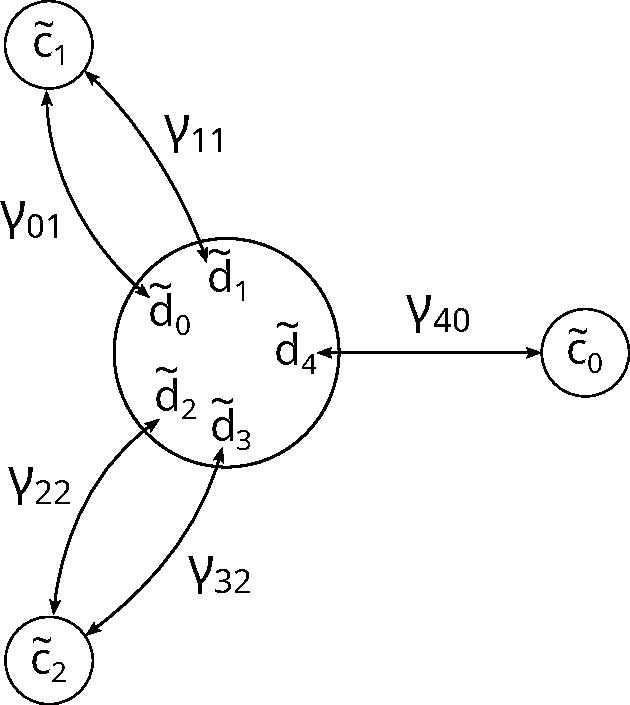
\includegraphics[width = 0.34\textwidth]{Plots/3band.pdf}
    \caption{Effektives Drei-Bänder Modell in dem die
    Vernichter $\tilde{d}_m$ und $\tilde{c}_l$ mit den Kopplungsstärken
    $\gamma_{ml}$ (Gl. \eqref{eqn:gammakop}) koppeln.
    Die Anordnug verdeutlicht nur das Konzept und entspricht nicht der 
    Anordnung im Realraum.}
    \label{fig:3band}
\end{wrapfigure}
In Gleichung \eqref{eqn:Hkopnice} zeigt sich welche Operatoren $\tilde{d}_m$ an welche Vernichter $\tilde{c}_l$ koppeln.
An den Vernichter $\tilde{c}_{0}$ koppelt nur ein einziger Vernichter, $\tilde{d}_{4}$, während an den Vernichter $\tilde{c}_{1}$ zwei Linearkobminationen der $3d$-Orbitale koppeln, nämlich 
die Vernichter $\tilde{d}_{0}$ und $\tilde{d}_{1}$. 
Die beiden übrigen Vernichter $\tilde{d}_{2}$ und $\tilde{d}_{3}$ koppeln an den Vernichter  $\tilde{c}_{2}$.
In der damit beschriebenen Situation liegt ein effektives Drei-Bänder Modell vor.
In den Hamiltonian $H_\text{Def}$ aus Gleichung \eqref{eqn:full_Hamiltonian} werden die alten Vernichter $d_m$ durch die neuen Vernichter $\tilde{d}_m$ unter 
der Annahme, dass die Orbitalenergie $\varepsilon_m$ für alle $3d$-Orbitale des Mn gleich ist, ersetzt, so dass sich der volle Hamiltonian $H$
aus Gleichung \eqref{eqn:full_Hamiltonian} mit der Beschreibung des ungestörten Graphens $H_0$, 
der Orbitale des Mn in der neuen Basis $H_{\text{Def}}$ mit der Orbitalenergie $\epsilon$ und
der Hybridisierung zwischen dem Mn und den drei umliegenden C mit $H_\text{Kop}$ in der neuen Basis zu\\
\\
\begin{align}
    H = -t\sum_{ij}(c^\dagger_i c_j + c^\dagger_j c_i) + \varepsilon \sum_{m=0}^4 \tilde{d}^\dagger_m \tilde{d}_m +
    \sum_{m=0}^4\sum_{l=0}^2(\gamma_{mj} \tilde{d}^\dagger_m \tilde{c}_l + \gamma_{ml} \tilde{c}^\dagger_l \tilde{d}_m) \; .
\end{align}
ergibt.
Dabei beinhaltet die Matrix $\underline{\underline{\gamma}}$ die Kopplungsstärken der Operatoren $\tilde{d}_m$ und $\tilde{c}_l$.
Diese ist mit $m \in \{ 0,1,2,3,4 \}$ und $l \in \{ 0,1,2 \}$ durch
\begin{equation*}
     \underline{\underline{\gamma}} = 
    \begin{pmatrix}
        0               & \left ( \frac{3}{\sqrt{8}} b V_{pd\sigma} + \frac{\sqrt{3}}{\sqrt{2}}  b   V_{pd\pi} \right )    &   0           \\
        0               & \left ( \frac{3}{\sqrt{2}} f V_{pd\sigma} + \frac{\sqrt{3}}{\sqrt{2}}  h   V_{pd\pi} \right )   &   0           \\
        0               & 0             &   \left ( \frac{3}{\sqrt{8}} b V_{pd\sigma} + \frac{\sqrt{3}}{\sqrt{2}}  b   V_{pd\pi} \right ) \\
        0               & 0             &   \left ( \frac{3}{\sqrt{2}} f V_{pd\sigma} + \frac{\sqrt{3}}{\sqrt{2}}  h   V_{pd\pi} \right ) \\
        \left (  \sqrt{3} q V_{pd\sigma} + 3 b V_{pd\pi} \right )     & 0             &   0           \\
    \end{pmatrix}
\end{equation*} \label{eqn:gammakop}
gegeben.
Um nun die gesuchte Hybridisierungsfunktion $\underline{\underline{\symup{\Delta}}}$ zu erhalten, werden die Greenschen Funktionen
$G_{\tilde{c}_l, \tilde{c}_l^{\dagger}}$ des ungestörten Graphens, welche mittels Rücktransformation der Greenschen Funktion 
$G_{c_{\text{B}, \vec{k}}, c_{\text{B}, \vec{k}}^\dagger}$ ermittelt werden können, benötigt.
Da der Einfluss des Mn mit der Systemgröße $N$ asymptotisch gegen 0 geht, ist die Verwendung der 
Greenschen Funktionen des Graphens ohne Störstelle gerechtfertigt.
Der Hamiltonian des ungestörten Graphens $H_0$ kann aus der Gleichung \eqref{eqn:full_Hamiltonian} übernommen werden,
worin die Fourier-transformierten Vernichter $c_i$ und $c_j$ (siehe Gleichung \eqref{eqn:fourier_ladder}) eingesetzt werden,
so dass sich der Hamiltonian $H_0$ zu  
\begin{equation}
    H = -t \sum_{\vec{k}}\sum_{j=1}^3( \symup{e}^{\symup{i}\vec{k}\vec{\delta}_j}c^\dagger_{\text{A},\vec{k}} c_{\text{B},\vec{k}} + \symup{e}^{-\symup{i}\vec{k}\vec{\delta}_j}c^\dagger_{\text{B},\vec{k}} c_{\text{A},\vec{k}} ) \; .
\end{equation} 
ergibt.
Um die Greensche Funktion $G_{c_{\text{B}, \vec{k}}, c_{\text{B}, \vec{k}}^\dagger}$ mit Hilfe der Bewegungsgleichung \eqref{eqn:fouriereom} zu bestimmen, werden die Kommutatoren
\begin{align}
    \left [H,  c_{\text{B},\vec{k}} \right ] &= t \sum_j \symup{e}^{-\symup{i}\vec{k}\vec{\delta}_j} c_{\text{A},\vec{k}} \label{eqn:test} \\
    \left [H,  c_{\text{A},\vec{k}} \right ] &= t \sum_j \symup{e}^{\symup{i}\vec{k}\vec{\delta}_j} c_{\text{B},\vec{k}}
\end{align}
benötigt (für explizite Berechung siehe Abschnitt \ref{sec:calc_greensfunction}).
Somit ergeben sich die Greenschen Funktionen
\begin{align}
    G_{c_{\text{A},\vec{k}}, c^\dagger_{\text{B},\vec{k}}} &=  \frac{t\sum_j \symup{e}^{\symup{i}\vec{k}\vec{\delta}_j}}{z} G_{c_{\text{B},\vec{k}}, c^\dagger_{\text{B},\vec{k}}}\\
    zG_{c_{\text{B},\vec{k}}, c^\dagger_{\text{B},\vec{k}}} &= 1 -  t\sum_j \symup{e}^{-\symup{i}\vec{k}\vec{\delta}_j} G_{c_{\text{A},\vec{k}}, c^\dagger_{\text{B},\vec{k}}} \; . \label{eqn:GreenBB}
\end{align}
Fortan wird $G_{c_{\text{A},\vec{k}}, c^\dagger_{\text{B},\vec{k}}}$ in die Gleichung \eqref{eqn:GreenBB} eingesetzt, womit
\begin{align}
    zG_{c_{\text{B},\vec{k}}, c^\dagger_{\text{B},\vec{k}}} &= 1 - \frac{t^2\sum_j \symup{e}^{-\symup{i}\vec{k}\vec{\delta}_j} \sum_{j'} \symup{e}^{\symup{i}\vec{k}\vec{\delta}_{j}} }{z} G_{c_{\text{B},\vec{k}}, c^\dagger_{\text{B},\vec{k}}} \\
    \iff G_{c_{\text{B},\vec{k}}, c^\dagger_{\text{B},\vec{k}}} &= \frac{z}{z^2 - \varepsilon^2_{\vec{k}}  } \; 
\end{align}
folgt. 
Dabei tritt die Dispersionsrelation von Graphen $\varepsilon_{\vec{k}}$ (siehe Gleichung \eqref{eqn:dispersion_graphene_calc}) auf. 
Um nun die gesuchte Greensche Funktion $G_{\tilde{c}_l, \tilde{c}_l^{\dagger}}$ zu erhalten, wird mit 
\begin{equation}
    G_{\tilde{c}_l, \tilde{c}^\dagger_{l'}} = \sum_{\vec{k}} D_{l,\vec{k}} D^\dagger_{l',\vec{k}}G_{c_{\text{B},\vec{k}}, c^\dagger_{\text{B},\vec{k}}} \label{eqn:koe}
\end{equation}
die Greensche Funktion $G_{c_{\text{B},\vec{k}}, c^\dagger_{\text{B},\vec{k}}}$ zurücktransformiert.
Die dabei auftretenden Koeffizienten $D_{l,\vec{k}}$ von den Fouriertransformationen der Vernichter $\tilde{c}_l$
\begin{align*}
    \tilde{c}_0 &= \frac{1}{\sqrt{3N}}\sum_{\vec{k}} \sum_{j=1}^3\symup{e}^{\symup{i}{\vec{k}}(\vec{l}+\vec{\delta}_j)}                              c_{\text{B}, \vec{k}}  \\
    \tilde{c}_1 &= \frac{1}{\sqrt{3N}}\sum_{\vec{k}} \sum_{j=1}^3\symup{e}^{\symup{i}{\vec{k}}(\vec{l}+\vec{\delta}_j)+\symup{i}\frac{2(j-1)\pi}{3}} c_{\text{B}, \vec{k}}  \\
    \tilde{c}_2 &= \frac{1}{\sqrt{3N}}\sum_{\vec{k}} \sum_{j=1}^3\symup{e}^{\symup{i}{\vec{k}}(\vec{l}+\vec{\delta}_j)-\symup{i}\frac{2(j-1)\pi}{3}} c_{\text{B}, \vec{k}}  
\end{align*}
sind durch
\begin{equation}
    \begin{aligned}
    D_{0,\vec{k}} &= \frac{1}{\sqrt{3N}}\sum_{j=1}^3\symup{e}^{\symup{i}{\vec{k}}(\vec{l}+\vec{\delta}_j)} \\
    D_{1,\vec{k}} &= \frac{1}{\sqrt{3N}}\sum_{j=1}^3\symup{e}^{\symup{i}{\vec{k}}(\vec{l}+\vec{\delta}_j)+\symup{i}\frac{2(j-1)\pi}{3}}  \\
    D_{2,\vec{k}} &= \frac{1}{\sqrt{3N}}\sum_{j=1}^3\symup{e}^{\symup{i}{\vec{k}}(\vec{l}+\vec{\delta}_j)-\symup{i}\frac{2(j-1)\pi}{3}}  \label{eqn:fourierko}
    \end{aligned}    
\end{equation}
gegeben.
Werden diese nun in \eqref{eqn:koe} eingesetzt, ergeben sich die 3 gesuchten Greenschen Funktionen zu 
\begin{align}
    G_{\tilde{c}_0, \tilde{c}^\dagger_0} &= \frac{z}{3N} \sum_{\vec{k}} \frac{\sum_j \symup{e}^{i{\vec{k}}\vec{\delta}_j} \sum_{j'} \symup{e}^{-i{\vec{k}}\vec{\delta}_{j'}}                                                            }{z^2-\varepsilon_{\vec{k}}^2} \\
    G_{\tilde{c}_1, \tilde{c}^\dagger_1} &= \frac{z}{3N} \sum_{\vec{k}} \frac{\sum_j \symup{e}^{i{\vec{k}}\vec{\delta}_j+\symup{i}\frac{2(j-1)\pi}{3}} \sum_{j'} \symup{e}^{-i{\vec{k}}\vec{\delta}_{j'}-\symup{i}\frac{2(j'-1)\pi}{3}} }{z^2-\varepsilon_{\vec{k}}^2} \\
    G_{\tilde{c}_2, \tilde{c}^\dagger_2} &= \frac{z}{3N} \sum_{\vec{k}} \frac{\sum_j \symup{e}^{i{\vec{k}}\vec{\delta}_j-\symup{i}\frac{2(j-1)\pi}{3}} \sum_{j'} \symup{e}^{-i{\vec{k}}\vec{\delta}_{j'}+\symup{i}\frac{2(j'-1)\pi}{3}} }{z^2-\varepsilon_{\vec{k}}^2} \; .
\end{align}
Da zweimal nur zwei Vernichter $\tilde{d}_m$ an einen Vernichter $\tilde{c}_l$ und einmal ein Operator $\tilde{d}_m$ an einen Operator $\tilde{c}_l$ koppeln
(siehe \eqref{eqn:Hkopnice}), 
besitzt die Hybridisierungsfunktion
eine blockdiagonale Struktur mit zwei $2 \times 2$-Blöcke und einem $1 \times 1$-Block auf der Hauptdiagonale, welche 
durch Multiplikation der Kopplungsparameter $\gamma_{ml}$ mit der zu dem $m$ zugehörige Greensche Funktion $G_{\tilde{c}_l, \tilde{c}^\dagger_{l'}}$ gegeben sind.
Somit kann die gesuchte Hybridisierungsfunktion $\underline{\underline{\symup{\Delta}}}$ zu
%\begin{equation}
%    (\underline{\underline{\symup{\Delta}}})_{mn} = 
%    \begin{pmatrix}
%        \gamma_{01}^2           G_{\tilde{c}_1, \tilde{c}^\dagger_1}        & \gamma_{01}\gamma_{11}  G_{\tilde{c}_1, \tilde{c}^\dagger_1}      & 0                                                                 & 0                                                             & 0                                                             \\
%        \gamma_{01}\gamma_{11}  G_{\tilde{c}_1, \tilde{c}^\dagger_1}        & \gamma_{11}^2           G_{\tilde{c}_1, \tilde{c}^\dagger_1}      & 0                                                                 & 0                                                             & 0                                                             \\
%        0                                                                   & 0                                                                 & \gamma_{22}^2           G_{\tilde{c}_2, \tilde{c}^\dagger_2}      & \gamma_{22}\gamma_{32}  G_{\tilde{c}_2, \tilde{c}^\dagger_2}   & 0                                                             \\
%        0                                                                   & 0                                                                 & \gamma_{22}\gamma_{32}  G_{\tilde{c}_2, \tilde{c}^\dagger_2}      & \gamma_{32}^2          G_{\tilde{c}_2, \tilde{c}^\dagger_2}   & 0                                                             \\
%        0                                                                   & 0                                                                 & 0                                                                 & 0                                                             & \gamma_{40}^2           G_{\tilde{c}_0, \tilde{c}^\dagger_0}  \\
%    \end{pmatrix}
%\end{equation}
\[
\begin{bmatrix}
    \begin{bmatrix}
        \gamma_{01}^2           & \gamma_{01}\gamma_{11}                \\
        \gamma_{01}\gamma_{11}  & \gamma_{11}^2                         \\
    \end{bmatrix} G_{\tilde{c}_1, \tilde{c}^\dagger_1}   &   \mathbf{0}  &   \mathbf{0}            \\
    \mathbf{0}      & \begin{bmatrix}
                        \gamma_{22}^2           & \gamma_{22}\gamma_{32}\\
                        \gamma_{22}\gamma_{32}  & \gamma_{32}^2         \\
                      \end{bmatrix} G_{\tilde{c}_2, \tilde{c}^\dagger_2}  &   \mathbf{0}          \\
    \mathbf{0}      &   \mathbf{0}  &   \gamma_{40}^2           G_{\tilde{c}_0, \tilde{c}^\dagger_0}       \\
\end{bmatrix}
\]
angegeben werden.
%Fouriertrafo für neue $\tilde{c}_i$ : 
%\begin{align*}
%    \tilde{c}_0 &= \frac{1}{\sqrt{3N}}\sum_{j\vec{k}}\symup{e}^{i{\vec{k}}(\vec{l}+\vec{\delta}_j)}                              c_{\text{B}, \vec{k}}  \\
%    \tilde{c}_1 &= \frac{1}{\sqrt{3N}}\sum_{j\vec{k}}\symup{e}^{i{\vec{k}}(\vec{l}+\vec{\delta}_j)+\symup{i}\frac{2(j-1)\pi}{3}} c_{\text{B}, \vec{k}}  \\
%    \tilde{c}_2 &= \frac{1}{\sqrt{3N}}\sum_{j\vec{k}}\symup{e}^{i{\vec{k}}(\vec{l}+\vec{\delta}_j)-\symup{i}\frac{2(j-1)\pi}{3}} c_{\text{B}, \vec{k}}  
%\end{align*}
%\begin{align*}
%    H = &-t \sum_{\vec{k}}\sum_{j=1}^3  ( \symup{e}^{i\vec{k}\vec{\delta}_j}c^\dagger_{A,\vec{k}} c_{B,\vec{k}} + 
%    \symup{e}^{-i\vec{k}\vec{\delta}_j} c^\dagger_{B,\vec{k}}c_{A,\vec{k}}) + 
%    \varepsilon \sum_{m=0}^4 \tilde{d}^\dagger_m \tilde{d}_m \\
%    &+\frac{1}{\sqrt{3N}} \sum_{\vec{k}} \sum_{m=0}^4 \sum_{l=0}^2 \sum_{j=1}^3 
%    (\gamma_{ml} \symup{e}^{i{\vec{k}}(\vec{l}+\vec{\delta}_j)+(-1)^{(\delta_{m2}+\delta_{m3})}     i\frac{2(j-1)\pi}{3}(1-\delta_{m4})}\tilde{d}^\dagger_m c_{B,\vec{k}} \\
%    &+ \gamma_{mj}  \symup{e}^{-i{\vec{k}}(\vec{l}+\vec{\delta}_j)-(-1)^{(\delta_{m2}+\delta_{m3})} i\frac{2(j-1)\pi}{3}(1-\delta_{m4})} c^\dagger_{B,\vec{k}} \tilde{d}_m)
%\end{align*}
%Hybridisierungsfunktion gegeben durch 
%\begin{align*}
%    \symup{\Delta}_{mn} = \frac{z}{3N} \sum_{\vec{k}} \frac{\sum_{jl} \gamma_{ml} \symup{e}^{i{\vec{k}}(\vec{l}+\vec{\delta}_j)+(-1)^{(\delta_{m2}+\delta_{m3})}     i\frac{2(j-1)\pi}{3}(1-\delta_{m4})}
%    \sum_{j'l'} \gamma_{nl'} \symup{e}^{i{\vec{k}}(\vec{l}+\vec{\delta}_{j'})-(-1)^{(\delta_{n2}+\delta_{n3})}     i\frac{2(j'-1)\pi}{3}(1-\delta_{n4})} }
%    {z^2 - |\varepsilon_{\vec{k}}|^2}
%\end{align*}
%mit der Dispersionsrelation $\varepsilon^{\pm}_{\vec{k}} = \pm  t \sum_j\symup{e}^{\symup{i}\vec{k}\vec{\delta}_j} \sum_{j'}\symup{e}^{-\symup{i}\vec{k}\vec{\delta}_{j'}}$.
%%\begin{equation*}
%%    \underline{\underline{\symup{\Delta}}} = 
%%    \begin{pmatrix}
%%        \symup{\Delta}_{00}     & \symup{\Delta}_{01}   & 0                     & 0                     & 0                     \\
%%        \symup{\Delta}_{10}     & \symup{\Delta}_{11}   & 0                     & 0                     & 0                     \\
%%        0                       & 0                     & \symup{\Delta}_{22}   & \symup{\Delta}_{23}   & 0                     \\
%%        0                       & 0                     & \symup{\Delta}_{32}   & sec:calc_greensfunction\symup{\Delta}_{33}   & 0                     \\
%%        0                       & 0                         & 0                     & 0                 & \symup{\Delta}_{44}   \\
%%    \end{pmatrix}
%%\end{equation*}
\section{Einfluss der Höhe des Mn}
In diesem Abschnitt wird der Einfluss der Position des Mn auf die Vorfaktoren der SK-Integrale (SK-Integrale in Tabelle \ref{tab:slaterkosters}, Vorfaktoren in Gl. \eqref{eqn:Vorfaktoren}) beschrieben.
Dazu sind in Abbildung \ref{fig:Faktoreninz} diese Vorfaktioren in Abhängigkeit von der Höhe des Mn $z$ graphisch dargestellt.
\begin{figure}
    \centering
    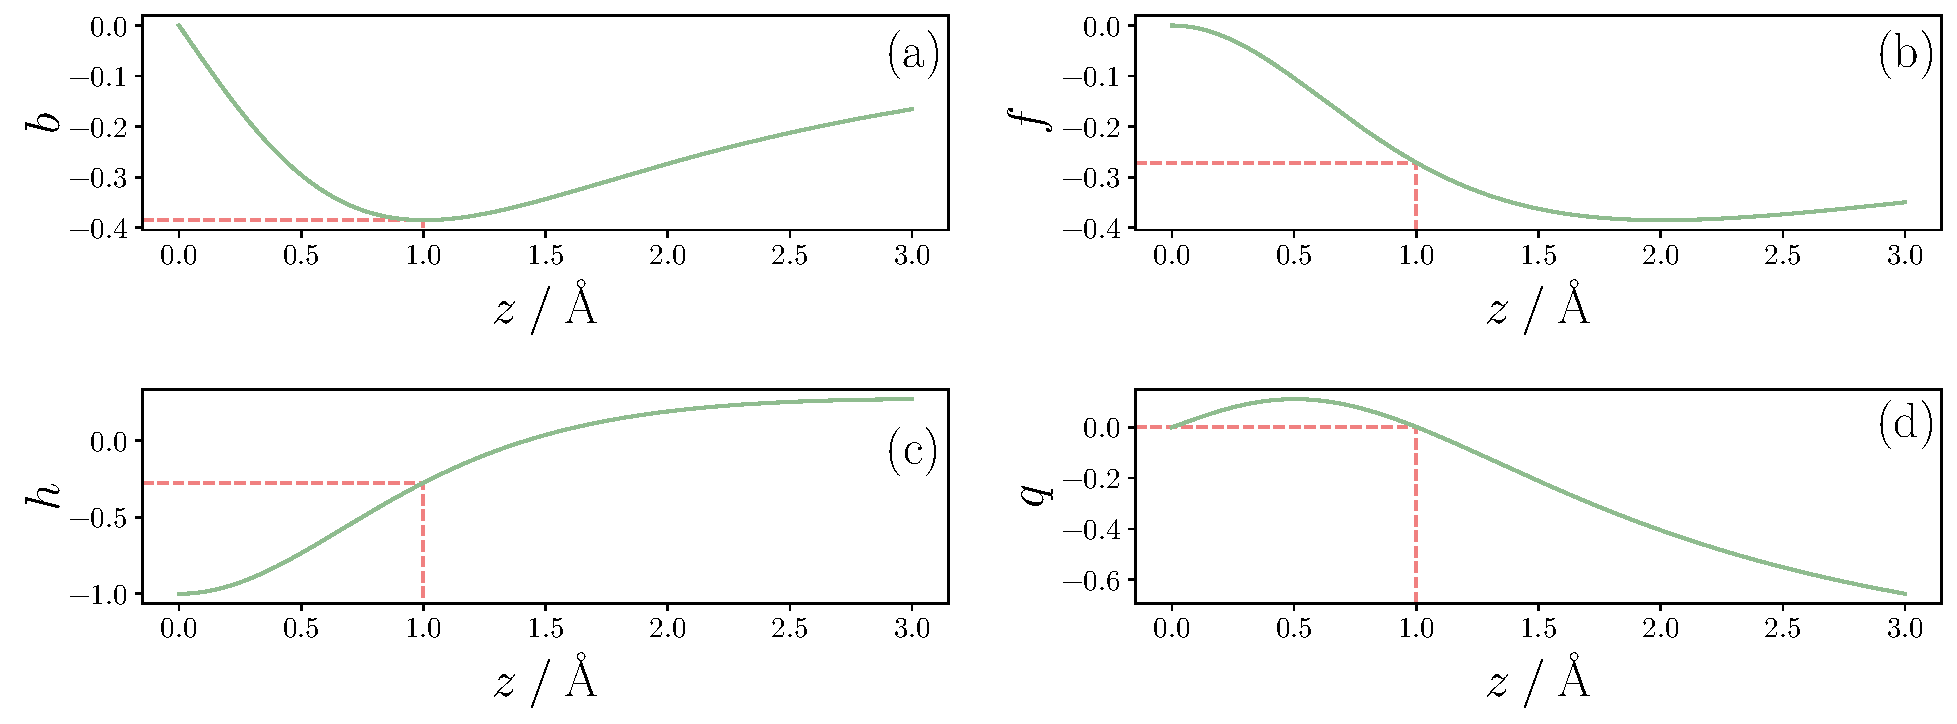
\includegraphics[width = \textwidth]{Plots/Faktoreninz.pdf}
    \caption{Vorfaktoren der SK-Integrale (Vorfaktoren in Gl. \eqref{eqn:Vorfaktoren}, SK-Integrale in Tabelle \ref{tab:slaterkosters}) in Abhängigkeit der der Höhe des Mn.
    Die Höhe varriert von $\qty{0}{\angstrom}$ (Mn in Graphenebene) bis $\qty{3}{\angstrom}$ (Mn in in der Ebene der Oberfläche des Kupfersubstrats).}
    \label{fig:Faktoreninz}
\end{figure}
Der Höhenbereich wurde in der Abbildung \ref{fig:Faktoreninz} auf $z \in [\qty{0}{\angstrom}, \qty{3}{\angstrom}]$ gewählt, da in dem Experiment aus dem Artikel \cite{doi:10.1021/acsnano.1c00139} 
der Abstand zwischen dem Graphen und dem Kupfersubstrat als ca. $\qty{3}{\angstrom}$ identifiziert wurde, während das Mn einen Abstand von 
ca. $\qty{1}{\angstrom}$ zu dem Graphen hat, weswegen auch die Punkte bei $z = \qty{1}{\angstrom}$ extra markiert wurden.
Bei dem Parameter $b$ (Abb. \ref{fig:Faktoreninz}a) fällt auf, dass dieser bei einer Höhe $z = \qty{0}{\angstrom} $ den Wert null annimmt.
Daraus lässt sich schließen, dass das SK-Integral $E_{z,xy}$ für alle drei umliegenden C und somit die Kopplung mit 
dem $d_{xy}$-Orbital des Mn bei geringen Höhen verschwindend klein ist. 
Ebenfalls ist der Abstand von der Graphenebene $z=\qty{1}{\angstrom}$ bei dem Vorfaktor $q$ von Interesse (Abb. \ref{fig:Faktoreninz}d), da dieser dort den Wert null annimmt.
Zwar bildet $q$ nicht den einzigen Vorfaktor bei einem SK-Integral, jedoch ist dieser Fall prägnant, da $q=0$ genau bei dem Abstand gilt, 
bei welchem sich das Mn laut dem Arikel \cite{doi:10.1021/acsnano.1c00139} befindet.
In Abbildung \ref{fig:Faktoreninz}c wird ersichtlich, dass der Parameter $h$ für große Abstände sehr klein bleibt. 
Daraus kann gefolgert werden, dass der Anteil der Kopplungen ausgehend von den $\pi$-Bindungen bei dem SK-Integral $E_{z,zy}$ für die C-Atome, deren
SK-Integral $E_{z,zy}$ verschieden von Null ist, bei großen Abständen sehr gering ist.